\chapter{Introducción}
\label{cap:intro}

Este manual acompaña al paquete de simulación \code{rotary\_pendulum}, segundo experimento de la serie de sistemas de control tras el péndulo lineal~\cite{lineal}. Está organizado en dos partes:
\begin{itemize}
  \item \textbf{Parte teórica} (capítulos~\ref{cap:modelo}--\ref{cap:control}): modelo dinámico, análisis lineal, sensores y diseño de controladores.
  \item \textbf{Parte práctica} (capítulos~\ref{cap:simulink}--\ref{cap:practicas}): el modelo Simulink, la interfaz de código, la interfaz gráfica y una serie de prácticas guiadas.
\end{itemize}
La estructura, la convención de nombres y la interfaz son paralelas a las del péndulo lineal, de modo que lo aprendido allí se traslada casi sin cambios. Los resultados numéricos y todas las gráficas de este manual se han obtenido simulando el modelo Simulink del paquete (MATLAB R2025b) y se han contrastado con una réplica independiente en Python (apéndice~\ref{cap:validacion}).

\section{El sistema}

El péndulo rotacional, o \emph{péndulo de Furuta}~\cite{furuta1992}, es la versión giratoria del carro-péndulo. Un motor de corriente continua hace girar un brazo horizontal de longitud $L_r$. En el extremo del brazo hay un pivote, cuyo eje es el propio brazo, del que cuelga un péndulo de longitud $L_p$ que oscila libremente en el plano perpendicular al brazo (figura~\ref{fig:sistema}).

\begin{figure}[H]
\centering
% Oblique 3D sketch of the rotary (Furuta) pendulum: z up, arm in the xy plane.
\begin{tikzpicture}[x={(1cm,0cm)},y={(0.55cm,0.38cm)},z={(0cm,1cm)},>=Latex,scale=1.05,
  every node/.style={font=\small}]
\pgfmathsetmacro{\th}{-28}      % arm angle [deg]
\pgfmathsetmacro{\al}{28}       % pendulum angle [deg]
\pgfmathsetmacro{\Lr}{2.6}
\pgfmathsetmacro{\Lp}{2.9}
\pgfmathsetmacro{\tx}{\Lr*cos(\th)}
\pgfmathsetmacro{\ty}{\Lr*sin(\th)}
\pgfmathsetmacro{\ex}{\tx-\Lp*sin(\al)*sin(\th)}
\pgfmathsetmacro{\ey}{\ty+\Lp*sin(\al)*cos(\th)}
\pgfmathsetmacro{\ez}{\Lp*cos(\al)}
% base plate
\begin{scope}[canvas is xy plane at z=-2.9]
  \fill[gray!12] (-2.2,-2.6) rectangle (3.6,2.6);
  \draw[gray!50] (-2.2,-2.6) rectangle (3.6,2.6);
\end{scope}
% motor body (cylinder)
\begin{scope}[canvas is xy plane at z=-2.9] \path coordinate (b1) at (-0.55,0) coordinate (b2) at (0.55,0); \end{scope}
\fill[c1!25!gray!60] (-0.55,0,-2.9) -- (-0.55,0,-0.35) -- (0.55,0,-0.35) -- (0.55,0,-2.9) -- cycle;
\begin{scope}[canvas is xy plane at z=-2.9]
  \fill[c1!25!gray!60] (0,0) circle (0.55);
\end{scope}
\draw[gray!60!black] (-0.55,0,-2.9) -- (-0.55,0,-0.35) (0.55,0,-2.9) -- (0.55,0,-0.35);
\begin{scope}[canvas is xy plane at z=-0.35]
  \fill[c1!15!gray!40,draw=gray!60!black] (0,0) circle (0.55);
\end{scope}
\node[white,font=\footnotesize\bfseries] at (0,0,-1.6) {DC};
% hub
\fill[gray!45] (-0.18,0,-0.35) rectangle (0.18,0,0);
% swept circle of the arm tip and theta reference
\begin{scope}[canvas is xy plane at z=0]
  \draw[gray,densely dotted] (0,0) circle (\Lr);
  \draw[gray] (0,0) -- (\Lr+0.5,0) node[pos=1,right,black]{$\theta=0$};
  \draw[->,c4,thick] (2.0,0) arc (0:\th:2.0);
  \node[c4] at ({2.45*cos(\th/2)},{2.45*sin(\th/2)}) {$\theta$};
\end{scope}
% shadow of the pendulum on the plate
\draw[gray!35,line width=3.5pt,line cap=round] (0,0,-2.9) -- (\tx,\ty,-2.9);
\draw[gray!45,line width=2.2pt,line cap=round] (\tx,\ty,-2.9) -- (\ex,\ey,-2.9);
% upright reference at the arm tip
\draw[gray,dashed] (\tx,\ty,0) -- (\tx,\ty,\Lp+0.3);
% arm
\draw[line width=5pt,c1,line cap=round] (0,0,0) -- (\tx,\ty,0);
\node[c1,anchor=south east] at (-0.15,0,0.2) {brazo $L_r$};
% pendulum
\draw[line width=3.5pt,c2,line cap=round] (\tx,\ty,0) -- (\ex,\ey,\ez);
\fill[c2] (\ex,\ey,\ez) circle (0.12);
\fill[white,draw=black] (\tx,\ty,0) circle (0.07);
\node[c2,right] at ({0.5*(\tx+\ex)+0.15},{0.5*(\ty+\ey)},{0.5*\ez}) {péndulo $L_p$};
% alpha arc (in the plane of the pendulum)
\draw[->,c4,thick] plot[domain=0:\al,samples=12]
  ({\tx-1.3*sin(\x)*sin(\th)},{\ty+1.3*sin(\x)*cos(\th)},{1.3*cos(\x)});
\node[c4] at ({\tx-1.75*sin(\al/2)*sin(\th)},{\ty+1.75*sin(\al/2)*cos(\th)},{1.75*cos(\al/2)}) {$\alpha$};
% motor voltage
\draw[->,thick] (-2.0,0,-1.6) -- (-0.65,0,-1.6) node[pos=0,left]{$V$};
% axes
\draw[->,gray] (-1.9,-2.1,-2.9) -- (-0.9,-2.1,-2.9) node[right]{$x$};
\draw[->,gray] (-1.9,-2.1,-2.9) -- (-1.9,-1.1,-2.9) node[above]{$y$};
\draw[->,gray] (-1.9,-2.1,-2.9) -- (-1.9,-2.1,-1.9) node[above]{$z$};
\end{tikzpicture}

\caption{Péndulo rotacional. El motor gira el brazo un ángulo $\theta$ en el plano horizontal; el péndulo forma un ángulo $\alpha$ con la vertical en el plano perpendicular al brazo.}
\label{fig:sistema}
\end{figure}

Frente al péndulo lineal hay tres diferencias importantes:
\begin{enumerate}
  \item \textbf{No hay raíl}: el brazo puede girar indefinidamente, así que no existen topes físicos. Solo un corte de seguridad (por los cables) limita $|\theta|$ a una vuelta.
  \item \textbf{La entrada es una tensión}, no una fuerza. El motor introduce una fuerza contraelectromotriz que actúa como un amortiguamiento viscoso adicional sobre el brazo.
  \item \textbf{La dinámica es más rica}: al girar el brazo aparecen términos centrípetos y de Coriolis que acoplan ambos ejes y que no existen en el carro-péndulo.
\end{enumerate}

Igual que en el péndulo lineal, \textbf{solo se miden ángulos}: un encoder en el eje del motor mide $\theta$ y otro en el pivote mide $\alpha$. Las velocidades las estima el controlador.

\begin{table}[H]
\centering\small
\begin{tabular}{@{}lll@{}}
\toprule
Símbolo & Significado & Convenio\\
\midrule
$\theta$ & ángulo del brazo [rad] & positivo antihorario visto desde arriba; no se envuelve\\
$\alpha$ & ángulo del péndulo [rad] & $0$ = arriba, $\pi$ = colgando; $\alpha>0$ se inclina hacia $+\theta$\\
$V$ & tensión del motor [V] & $V>0$ acelera el brazo hacia $+\theta$; saturación $\pm\SI{10}{V}$\\
$\vect s$ & estado & $[\theta,\ \thd,\ \alpha,\ \ald]^\top$\\
\bottomrule
\end{tabular}
\caption{Variables y convenio de signos.}
\label{tab:convenio}
\end{table}

\begin{nota}
La interfaz de código trabaja en \textbf{radianes}. La interfaz gráfica y los campos \code{*\_deg} de los resultados (\code{th\_deg}, \code{al\_deg}, \code{r\_deg}) usan grados.
\end{nota}

\section{Contenido del paquete}

\begin{table}[H]
\centering\small
\begin{tabularx}{\linewidth}{@{}lX@{}}
\toprule
Archivo & Contenido\\
\midrule
\code{rp\_params.m} & Parámetros físicos, del motor, de los sensores y de los controladores.\\
\code{rp\_linearize.m}, \code{rp\_lqr.m}, \code{rp\_design.m} & Linealización, LQR (con o sin toolbox) y cálculo de inercias y ganancias.\\
\code{rp\_plant\_block.m} & Dinámica no lineal con motor (código del bloque \emph{MATLAB Function} de la planta).\\
\code{rp\_controller\_block.m} & Controlador discreto con 5 modos (código del bloque del controlador).\\
\code{rp\_ref\_block.m} & Generador de referencias del brazo.\\
\code{rp\_build\_model.m} & Genera el modelo \code{rotpend\_sim.slx} mediante un script.\\
\code{RotaryPendulum.m} & Clase con la interfaz de código: ensayos por lotes y control en vivo.\\
\code{rp\_gui.m} & Interfaz gráfica en vivo con animación 3D.\\
\code{rp\_draw.m}, \code{rp\_view.m}, \code{rp\_animate.m}, \code{rp\_plot\_results.m} & Escena 3D, puntos de vista, reproducción de ensayos y gráficas.\\
\code{examples.m} & Recorrido guiado por secciones.\\
\code{python\_reference\_sim.py} & Réplica independiente en Python usada para validar el modelo.\\
\code{validation/} & Scripts de validación cruzada Simulink--Python (apéndice~\ref{cap:validacion}).\\
\bottomrule
\end{tabularx}
\caption{Archivos del paquete \code{rotary\_pendulum}.}
\label{tab:archivos}
\end{table}

\section{Requisitos y puesta en marcha}

Se necesita MATLAB y Simulink R2020b o posterior (se ha probado con R2025b). La Control System Toolbox es opcional: si no está instalada, \code{rp\_lqr} resuelve la ecuación de Riccati por el método del Hamiltoniano, igual que en el péndulo lineal.

\begin{lstlisting}[caption={Primeros pasos.}]
cd src/rotary_pendulum
rp_build_model                 % crea rotpend_sim.slx (solo la primera vez)
rp_gui                         % interfaz gráfica en vivo
% o desde código:
rp = RotaryPendulum();
rp.setInitialState([0 0 pi 0]);   % péndulo colgando
rp.setMode('swingup');
res = rp.run(8);
rp_plot_results(res); rp.animate(res);
\end{lstlisting}

La figura~\ref{fig:frames} muestra la animación de ese ensayo: el controlador bombea energía al péndulo con movimientos alternos del brazo y lo captura arriba a los \SI{1.89}{s}.

\begin{figure}[H]
\centering
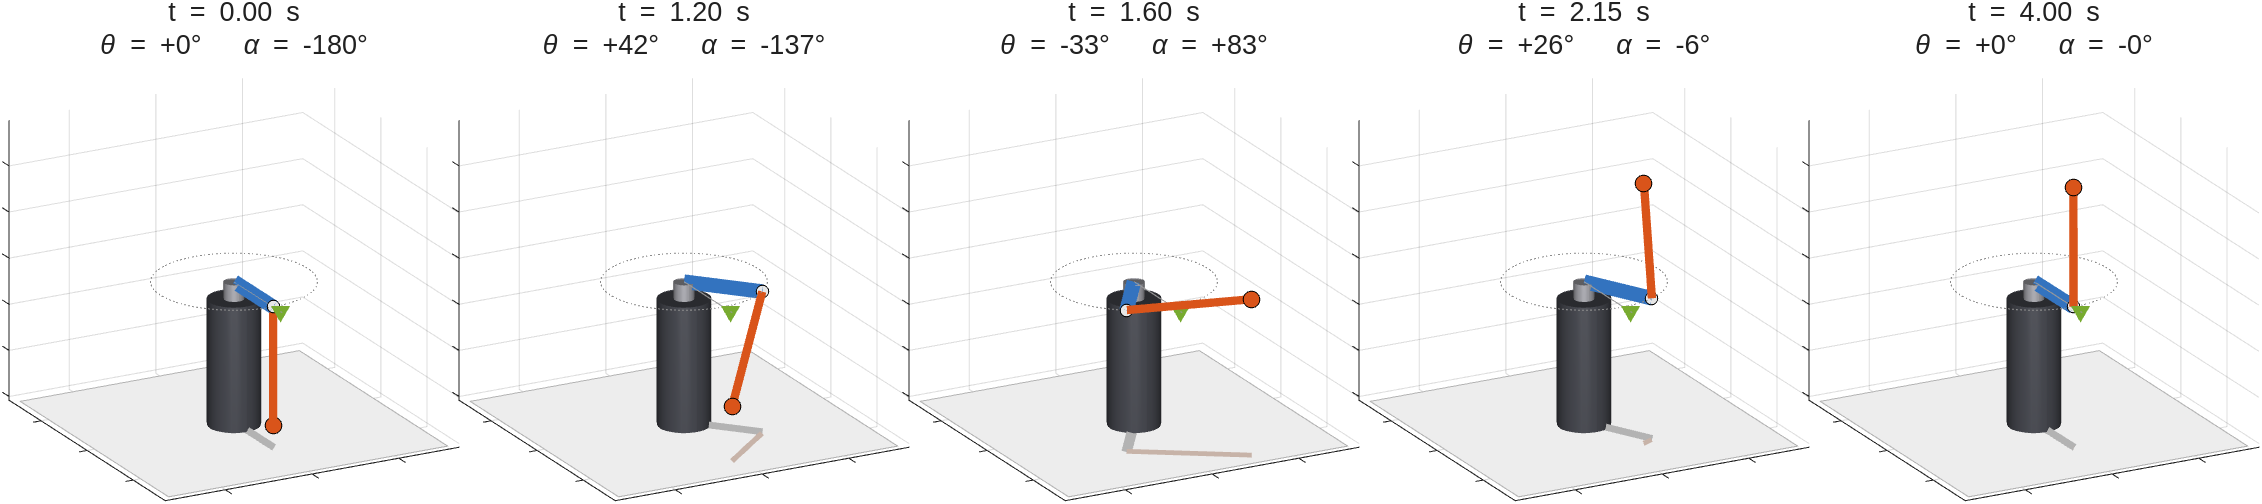
\includegraphics[width=\linewidth]{data/frames.png}
\caption{Fotogramas de la animación 3D (\code{rp\_animate}) durante un swing-up desde el reposo colgando. Las sombras sobre la base ayudan a percibir la profundidad; el triángulo verde marca la referencia del brazo.}
\label{fig:frames}
\end{figure}
